


\section{Numerical Analysis}

In order to validate the approximations made in previous sections, we solve system \ref{eq:system} numerically. In order to do so, we use the Runge-Kutta Method of order 4 along with the  Shooting Method to solve the two point boundary value (reference to Numerical Methods in python).  



The complexity of the problem lies exactly in the two point boundary feature of the problem, where the concentrations are known in the bulk, but the potential is known at the interface(see Fig. \ref{fig:geometry}). 

The approach used in these type of problems is transforming the second order system \ref{eq:system} into a first order one,

\begin{eqnarray}
C'_+(x)-\frac{zF}{RT}E(x)C_+(x) &=& -r, \\
C'_-(x)+\frac{zF}{RT}E(x)C_-(x) &=& 0, \\
E'(x) &=& \frac{zF}{\epsilon}(C_+(x)-C_-(x)), \\
\phi'(x) &=& -E(x).
\label{eq:linear-system}
\end{eqnarray}

subject to the border conditions

\begin{eqnarray}
C_+(\delta) = C_b  \\
C_-(\delta) = C_b \\
\phi(\delta) &=& 0\\
\phi(0) &=&  V_0
\label{eq:linear-system}
\end{eqnarray}

Here the primes denote derivatives with respect to $x$. Once the system is in the form of Eqn. \ref{eq:linear-system}, we can apply the Runge-Kutta Method with the shooting method to obtain the numerical solutions. 

\subsection{Runge-Kutta Method}
\label{sec:run_kut}

The Runge-Kutta Method is used to determine the numerical value of a system of differential equations to which we know the boundary conditions. Let 

$$\vec{y}' = \vec{F}(x, \vec{y})$$
$$\vec{y}(x_0) = \vec{y}_0$$

be the system of equations we want to solve with the method. We approximate the derivative by

$$\frac{\vec{y}(x+h)-\vec{y}(x)}{h} = \vec{F}(x + h, \vec{y}+\vec{y}(x+h))$$

We want to approximate the left hand side with a series expansion to arbitrary order in $h$. We obtain thus an expression for $y(x+h)$,

$$\vec{y}(x+h)=\vec{y}(x)+ h\vec{F}(x + h, \vec{y}+\vec{y}(x+h)).$$

In this work we use the Runge-Kutta of fifth order in the integration step $h$. The expression for the increment at this order of precision is

$$\vec{y}_5(x+h) = \vec{y}(x) + \sum_{i=0}^{6} C_{i} K_i,$$

and

$$K_0 = hF(x,y),$$
$$K_i = hF(x+A_ih,y+\sum_{i=0}^{i-1} B_{ij} K_j)$$

where $i = 1,2,3, .. , 6 $.

We also need the fourth order Runge-Kutta method in order to obtain the error in the integration. This is given by

$$\vec{y}_4(x+h) = \vec{y}(x) + \sum_{i=0}^{6} D_{i} K_i,$$

The error is given by 

\begin{eqnarray}
\vec{E}(h) = \vec{y}_5(x+h) - \vec{y}_4(x+h).
\end{eqnarray}

Of this expression, we can take the root mean square of the components of $\vec{E}(h)$,

\begin{equation}
e(h) = \sqrt{\frac{1}{n}\sum_{i=0}^{n-1}E_i^2(h)}
\end{equation}

This way we obtain a scalar measure of the error.

If $h_1$ and $h_2$ are two consecutive steps in the integration of the differential equation, then it can be shown that

\begin{equation}
\frac{e(h_1)}{e(h_2)} \approx \qty{\frac{h_1}{h_2}}^5
\label{eq:error}
\end{equation}

We don't know what the error of the next step will be, but we can define a tolerance $\epsilon>0$ such that the error of the next step is at most $\epsilon$. Thus, the following step can be computed from Eq. \ref{eq:error} by letting $e(h_2) = \epsilon$

\begin{equation}
h_2= h_1\qty{\frac{\epsilon}{e(h_1)}}^{1/5}
\label{eq:error}
\end{equation}

This method is good for our purposes since the curves we are trying to analyze are flat at the begining but have sharp slopes towards the interface (see Fig. \ref{fig:concentration} and \ref{fig:firstorderphi}).

\subsection{The Shooting Method}

The method described in section \ref{sec:run_kut} can solve the system of equations if the border conditions are all known at a given value of $x = x_0$. Nevertheless, as it can be seen from \ref{eq:border-conditions},
that we have boundary conditions at $x=0$ (the interface) and at $x=\delta$ the bulk solution (see Fig. \ref{fig:geometry}). This is a complication which can be overcome by using the shooting method. The idea is to transform the problem with boundary conditions 

$$C_+(\delta) = C_-(\delta) = C_b$$
$$\phi(\delta) = 0$$
$$\phi(0) = V_0$$

into the problem


$$C_+(\delta) = C_-(\delta) = C_b$$
$$\phi(\delta) = 0$$
$$E(\delta) = u,$$

where $u$ is a constant yet to be determined. To determine $u$, we define a residual function

$$r(u) = \phi(0)-V_0.$$

which is zero when the valueof $\phi(0)$ (given an appropriate u) is the original boundary condition. Therefore, the two-point boundary problem is transformed into a  root finding problem. First, we need to find two values of $u$, $u_1$ and $u_2$ such that $r(u_1) < 0$ and  $r(u_2) > 0$. Once we have that, we can use Ridder's method to find the root.

\subsection{Ridder's Method}

In this method it is assumed that the root is bracketed within to values.  We define an auxiliary function 
$$G(x) = F(x)e^{(x-x1)Q}$$
where $Q$ is determined by imposing that the points $(x_1, G(x_1))$, $(x_2, G(x_2))$ and $(x_3, G(x_3))$ be in a straight line. That is, if $x_1-x_2 = 2h$ and f $x_1-x_3 = h = x_3-x_2$ we should get

\begin{equation}
G(x_3) = \frac{G(x_1)-G(x_2)}{2}.
\label{eq:line-requirement}
\end{equation}

Using equation \ref{eq:line-requirement}, we obtain that

\begin{eqnarray}
e^{hQ} = \frac{f(x_1)+f(x_2)e^{2hQ}}{2}
\end{eqnarray}

Which is a quadratic equation on $e^{hQ}$. Solving for this quantity we obtain

\begin{equation}
e^{hQ} = \frac{f(x_3)\pm\sqrt{f(x_3)^2-f(x_2)f(x_1)}}{f(x_2)}
\end{equation}

Now that we have determined completely our function $G(x)$, we can do linear interpolation on it to get a better estimation of the root of f(x). Let $x_r$  be it. Then

$$x_r^{\pm} = x_3 \pm (x_3-x_1)\frac{f(x_3)}{\sqrt{f^2(x_3)-f(x_1)f(x_2)}}$$

It can be show that 
\begin{itemize}
\item If $f(x_1)-f(x_2) < 0$, we should pick the $x_r^-$ solution
\item If $f(x_1)-f(x_2) > 0$, we should pick the $x_r^+$ solution
\end{itemize}

When we have our solution, we make $x_3 = x_r^{s}$ ($s+,-$, for every case) and find a new correction to $x_r$. We stop when $x_r^+-x_r^-$ is below the define tolerance.

To test convergence, out method assumes the function we are passing on is of the form

$$f(x) = g(x) -g_0,$$

where we are trying to find $x_0$ such that $g(x_0) = g_0$. This means that when the root is found, we should get 

$$f(x_0) \in [-\epsilon,+\epsilon],$$

where $\epsilon>0$ is a predefined tolerance.

\subsection{Results}

Figures \ref{fig:numerical_c} and \ref{fig:numerical-phi} show the results obtained. The tendency looks correct, since the concentration of $SO_4^{-2}$ drops rapidly close to the interface and the concentration of $Cu^{+2}$ explodes at the same location. The potential drops close to the value of $\bar{V}_0\approx -0.15 V$.

Dealing with the equations as presented in Eq. \ref{eq:system} is extremely difficult when doing a numerical analysis. This is due to the fact that the natural units of the system (x which is measured in meters) are too small for the computer to handle. Also, non-linearity gives extreme fluctuations of the concentration of the positive ion near the surface. Since we where using the shooting method, we needed to change the values of the electric field at the bulk, such that the boundary condition for the electric potential is correct, but this induced such strong concentrations at the interface sometimes, that the computer could not handle the numbers resulting from Runge-Kutta method. We had to make a little adaptation in order to be able to find the correct boundary condition for the electric field with the shooting method. 

\newpage
\begin{figure}[h!]
 \centering
  \includegraphics[width = 0.6\linewidth]{concentration-num}
 \caption{This figure shows the concentration found analytically and through numerical analysis.}
 \label{fig:numerical_c}
\end{figure}


As it can be seen in figures  \ref{fig:numerical-phi},  \ref{fig:numerical-E}, the electric field and potential approach zero when the start moving into the bulk of the solution, as expected. The further away from the interface we go, the better the border conditions for the electric field are met. For our particular case, we cut the integration range when we reached a tolerance of $ E_{bulk} < 1\times 10^{-3}$, where $E_{bulk}$ is the border condition of the dimensionless electric field at the bulk. 

\begin{figure}[h!]
 \centering
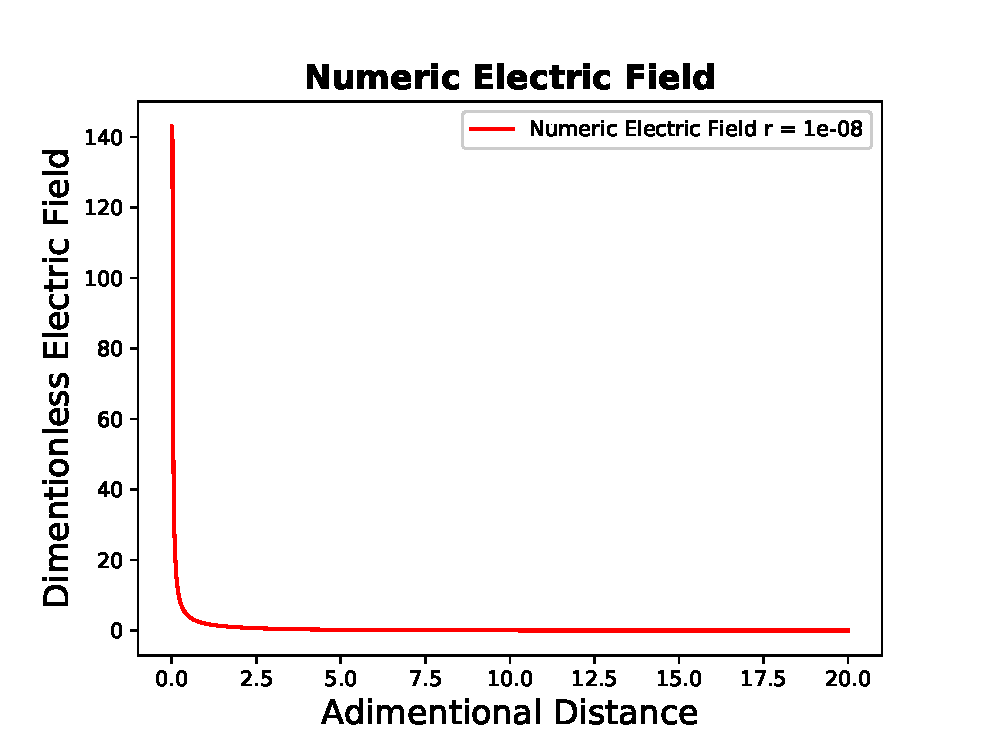
\includegraphics[width = 0.6\linewidth]{Efield-numeric}
 \caption{The numerical and the analytic electric field found with Runge-Kutta Method.}
 \label{fig:numerical-E}
\end{figure}


A similar analysis can be done for the concentrations (Fig.  \ref{fig:numerical_c}), but this time the value of both concentrations at the bulk is $C_b$, as defined by the border conditons for the system \ref{eq:system}.


\begin{figure}[h!]
 \centering
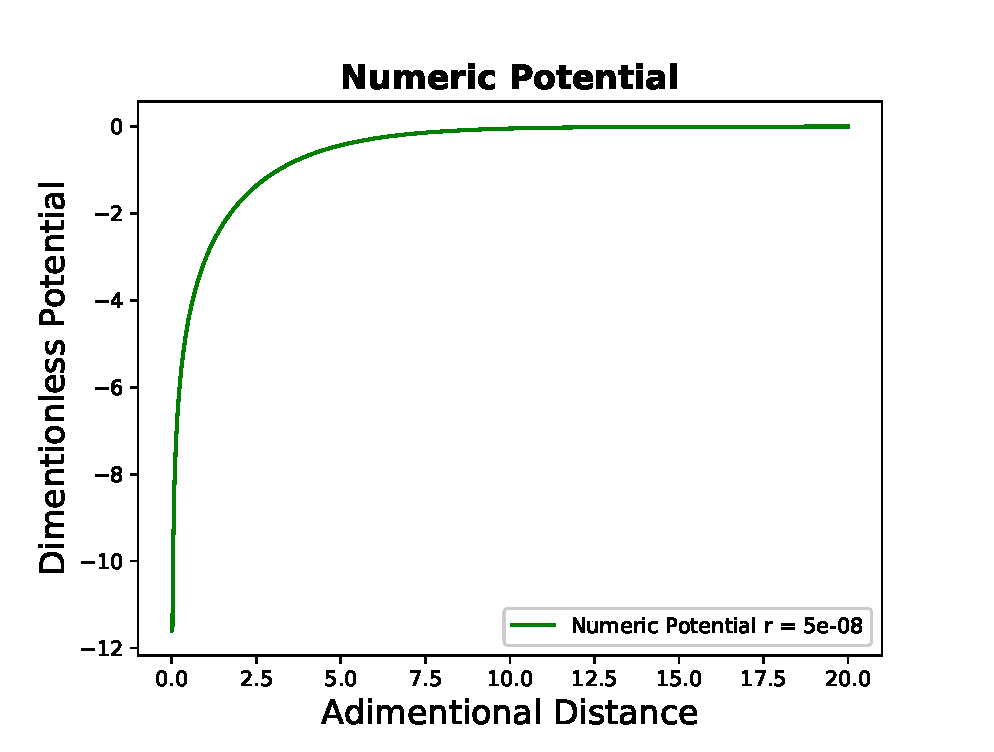
\includegraphics[width = 0.6\linewidth]{potential-num}
 \caption{The numerical and the analytic solution to the potential to first order in the current.}
 \label{fig:numerical-phi}
\end{figure}

Another difficulty is that, since we used the adaptive Runge-Kutta method, the concentrations change so abruptly that the adaptive step $h$ becomes increadibly small. The problem with this is that the number of iterations needed with a step of the order of $h\approx 10^{-29}$ to reach the full length of integration is too big and therefore, we obtain only a part of the integration interval and not as close to the interface as we should like. 

To avoid such difficulties, we have worked with the adimensional potential in a scale of adimensional length $\xi = \kappa x$. We have integrated on the interval $[0, 20 \kappa \delta]$.



\newpage

\section*{Comparing numeric an analytic results}

Fig. \ref{fig:numerical-phi} shows the comparison between the numeric and analytic results for the potential. In figures \ref{fig:results-c} to  \ref{fig:numerical-phi} there is a clear overestimation in the concentration of the positive ion, as well as an over estimation of the electric potential. This is due to the fact that we neglected the therm proportional to 

$$C_s \frac{\partial \phi^{(1)}}{\partial x}.$$ 


\begin{figure}[h!]
 \centering
\includegraphics[width = 0.6\linewidth]{concentration-results}
 \caption{Blue curves represent the concentration of the positive ion. Red curves represent the concentration of the negative ion. Dashed lines are numerical results and solid lines represent analytical results.}
 \label{fig:results-c}
\end{figure}


This is a good approximation when calculating the $C_-$ concentration, since it drops to zero near the interface. Since the $C_+$ concentration explodes near the interface, the approximation should be valid only to about $8\kappa$, as can be seen from Fig. \ref{fig:results-c}. Nevertheless, since $\phi^{(1)}$ is only a small contribution to the potential and by condition \ref{}, since $r$ is small, the approximation might be consider for even closer distances to the interface.


\begin{figure}[h!]
 \centering
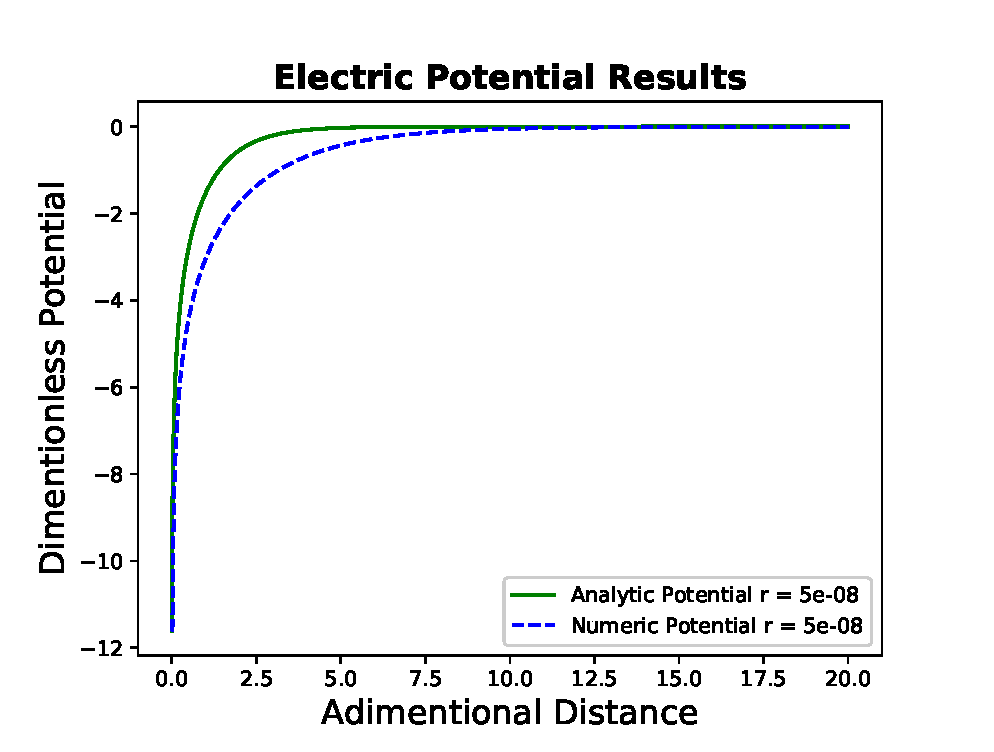
\includegraphics[width = 0.6\linewidth]{potential-results}
 \caption{Electric potential of the diffusion-reaction system subject to a non zero border condition for the potential. Dashed curve represents the numerical (exact) solution to system \ref{eq:system}, whereas the solid curve is the analytical solution obtained on section \ref{sec:analytic-result}. Screening due to positive ions gathering close to the interface is appreciated.}
 \label{fig:numerical-phi}
\end{figure}

The estimation for the Electric field, however, does look promising (Fig.  \ref{fig:numerical-phi}) . The analytical and numerical solutions of the model fit together particularly well the closer they get to the interface, even though both results explode  to really high values around this point.
\begin{figure}[h!]
 \centering
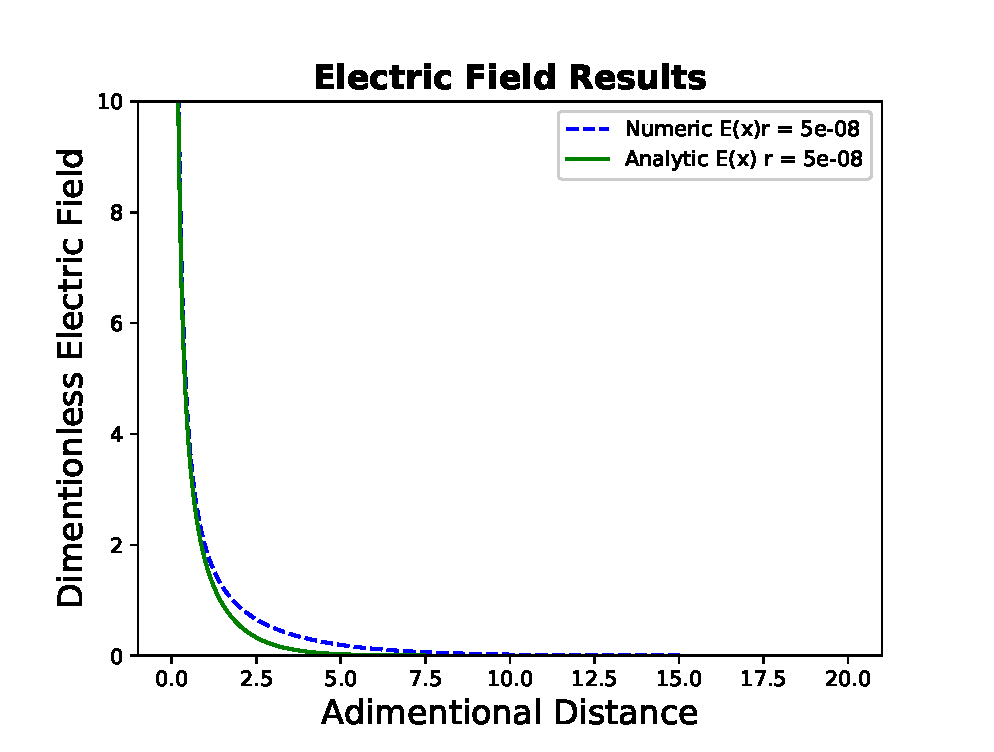
\includegraphics[width = 0.6\linewidth]{efield-results}
 \caption{The electric field is plotted comparing analytical (solid line) to numeric (dashed line) results.}
 \label{fig:numerical-phi}
\end{figure}




